%\documentclass[letterpaper,english,reprint,nofootinbib,aps,superscriptaddress,showpacs,showkeys]{revtex4-1}
\documentclass[pra,letterpaper,english,preprint,nofootinbib,aps,superscriptaddress,showkeys]{revtex4-1}

\usepackage{babel,calc,amsmath,amsthm,amssymb,graphicx,subfigure,xcolor,comment}
\usepackage{mathdots}
%\usepackage[notref,notcite,color]{showkeys}
\usepackage[T1]{fontenc}
\setcounter{secnumdepth}{3}
\usepackage[unicode=true]{hyperref}
\usepackage{booktabs}
\usepackage{threeparttable}
\usepackage{braket}
\usepackage{multirow}

\usepackage[normalem]{ulem}
\hypersetup{
     colorlinks=true,       		% false: boxed links; true: colored links
     linkcolor=blue,          	% color of internal links
     citecolor=red,             % color of links to bibliography
    % filecolor=blue,      		% color of file links
     urlcolor=black,          % color of external links
    % runcolor=cyan
 }
%% THEOREMS -------------------------------------------------------
\newtheorem{theorem}{Theorem}
\newtheorem*{theorem*}{Theorem}
\newtheorem{corollary}{Corollary}
\newtheorem*{corollary*}{Corollary}
\newtheorem{lemma}{Lemma}
\newtheorem*{lemma*}{Lemma}
\newtheorem{proposition}{Proposition}
\newtheorem*{proposition*}{Proposition}
\theoremstyle{definition}
\newtheorem{definition}{Definition}
\newtheorem*{definition*}{Definition}
\theoremstyle{remark}
\newtheorem{remark}{Remark}
\newtheorem*{remark*}{Remark}
%% MATH -----------------------------------------------------------
\newcommand{\norm}[1]{\left\Vert#1\right\Vert}
\newcommand{\abs}[1]{\left\vert#1\right\vert}

\newcommand{\Real}{\mathbb R}
\newcommand{\eps}{\varepsilon}
\newcommand{\To}{\longrightarrow}
\newcommand{\BX}{\mathbf{B}(X)}
\newcommand{\A}{\mathcal{A}}
%% ----------------------------------------------------------------
\newif\ifdebug

% \debugtrue

\ifdebug
\definecolor{zhliu}{rgb}{0.5, 0.03, 0}
\newcommand{\add}[1]{\textcolor{zhliu}{#1}}
\newcommand{\note}[1]{\textcolor{zhliu}{#1}}
\newcommand\delete{\bgroup\markoverwith{\textcolor{zhliu}{\rule[0.5ex]{2pt}{0.8pt}}}\ULon}
\newcommand{\replace}[2]{\delete{#1}\add{#2}}
\else
\newcommand{\add}[1]{#1}
\newcommand{\note}[1]{\ignorespaces}
\newcommand{\delete}[1]{\ignorespaces}
\newcommand{\replace}[2]{#2}
\fi

\newcommand{\tr}{\rm tr}
\newcommand{\rom}[1]{\MakeUppercase{\romannumeral #1}}


\begin{document}
\renewcommand{\figurename}{Fig.}

\title{Experimental Demonstration of Quantum Contextuality beyond Bell Nonlocality}


\author{Zheng-Hao Liu}
\affiliation{CAS Key Laboratory of Quantum Information, University of Science and Technology of China, Hefei 230026, People's Republic of China}
\affiliation{Synergetic Innovation Center of Quantum Information and Quantum Physics, University of Science and Technology of China, Hefei 230026, People's Republic of China}

\author{Hui-Xian Meng}
\affiliation{Theoretical Physics Division, Chern Institute of Mathematics, Nankai University, Tianjin 300071, People's Republic of China}

\author{Zhen-Peng Xu}
\affiliation{Theoretical Physics Division, Chern Institute of Mathematics, Nankai University, Tianjin 300071, People's Republic of China}

\author{Jie Zhou}
\affiliation{Theoretical Physics Division, Chern Institute of Mathematics, Nankai University, Tianjin 300071, People's Republic of China}

\author{Sheng Ye}
\affiliation{CAS Key Laboratory of Quantum Information, University of Science and Technology of China, Hefei 230026, People's Republic of China}
\affiliation{Synergetic Innovation Center of Quantum Information and Quantum Physics, University of Science and Technology of China, Hefei 230026, People's Republic of China}

\author{Qiang Li}
\affiliation{CAS Key Laboratory of Quantum Information, University of Science and Technology of China, Hefei 230026, People's Republic of China}
\affiliation{Synergetic Innovation Center of Quantum Information and Quantum Physics, University of Science and Technology of China, Hefei 230026, People's Republic of China}

\author{Kai Sun}
\affiliation{CAS Key Laboratory of Quantum Information, University of Science and Technology of China, Hefei 230026, People's Republic of China}
\affiliation{Synergetic Innovation Center of Quantum Information and Quantum Physics, University of Science and Technology of China, Hefei 230026, People's Republic of China}

\author{Jing-Ling Chen}
\email{chenjl@nankai.edu.cn}
\affiliation{Theoretical Physics Division, Chern Institute of Mathematics, Nankai University, Tianjin 300071, People's Republic of China}

\author{Jin-Shi Xu}
\email{jsxu@ustc.edu.cn}
\affiliation{CAS Key Laboratory of Quantum Information, University of Science and Technology of China, Hefei 230026, People's Republic of China}
\affiliation{Synergetic Innovation Center of Quantum Information and Quantum Physics, University of Science and Technology of China, Hefei 230026, People's Republic of China}

\author{Chuan-Feng Li}
\email{cfli@ustc.edu.cn}
\affiliation{CAS Key Laboratory of Quantum Information, University of Science and Technology of China, Hefei 230026, People's Republic of China}
\affiliation{Synergetic Innovation Center of Quantum Information and Quantum Physics, University of Science and Technology of China, Hefei 230026, People's Republic of China}

\author{Guang-Can Guo}
\affiliation{CAS Key Laboratory of Quantum Information, University of Science and Technology of China, Hefei 230026, People's Republic of China}
\affiliation{Synergetic Innovation Center of Quantum Information and Quantum Physics, University of Science and Technology of China, Hefei 230026, People's Republic of China}

\date{\today}

\begin{abstract}
Bell nonlocality is a type of quantum contextuality in which compatible measurements are, in addition, spacelike separated. As a consequence, the maximum quantum violation of a Bell inequality cannot be larger than the maximum quantum violation of a noncontextuality (NC) inequality that has the same exclusivity graph. 
However, the quantum violation of the NC inequality may be {\em larger} than the one of the Bell inequality with the same exclusivity graph. There exist NC inequalities with  larger quantum violations. 
We show that the maximum quantum violation of the NC inequality with the same exclusivity graph as \add{the Bell-type inequality} $I_{3322}$ is achieved with quantum systems of dimension five, and for \add{a} four-dimensional system the difference of maximum quantum violation of $I_{3322}$ for quantum contextuality and Bell nonlocality is larger than $0.3$. 
We experimentally test this difference. Within the experimental errors, the experimental results coincide with the theoretical predictions.
\end{abstract}

\pacs{03.65.Ud, 03.67.Mn, 42.50.Xa}

	\maketitle

\emph{Introduction.} ---A physical theory exhibits contextuality (or \replace{lack of}{lacks} noncontextuality) if measurement outcomes cannot be reproduced by models in which outcomes are independent of the measurement context (i.e., the set of jointly measurable observables actually measured). 
These models are called  noncontextual hidden variable (NCHV) models.
Similarly, a physical theory exhibits nonlocality (or lack of locality) if measurement outcomes cannot be reproduced by models in which measurement outcomes are independent of spacelike separated measurements. These models are those local hidden variable (LHV) models. 

% Kochen and Specker \cite{Specker60, KS67} (Bell) \cite{Bell66} proved that quantum theory (QT) does not admit NCHV (LHV) models. 
Contextuality and nonlocality are related concepts: both reflect \delete{a} conflict with models in which measurement outcomes are determined before measurements are performed. 
\add{Kochen and Specker \cite{Specker60, KS67} (Bell) \cite{Bell66} already ruled out NCHV (LHV) models from quantum theory (QT).}
\add{A bunch of inequalities regarding NCHV/LHV models are proposed, and their maximal violation values are governed by QT to preserve causality and uncertianty principle. \note{(add citation?)}}
However, a fundamental observation is that, \delete{in the case of QT, }the quantum nonlocality manifested in the violation of Bell inequalities \cite{Bell64} actually follows from the quantum contextuality manifested in the violation of noncontextuality (NC) inequalities \cite{KCBS08,Cabello08}. 
Every Bell inequality becomes a NC inequality \replace{the moment there is no spacelike separation between the compatible measurements}{if the constraint of spacelike separation between the compatible measurements is removed}.
\replace{Then}{So} all the applications of quantum nonlocality to quantum information are, in fact, applications of quantum contextuality in special scenarios. If we add the applications of quantum contextuality using noncomposite systems, \delete{then }the list of applications of quantum contextuality is rather impressive. 
It includes fault-tolerant computation \cite{Raussendorf13,HWVE13}, secret key distribution \cite{Ekert91,CDNS11}, reduction of communication complexity \cite{BZPZ04,BCMW10}, and randomness certification \cite{PAMBMMOHLMM10,UZZWYDDK13}.

A natural question is whether quantum contextuality may go {\em beyond} quantum nonlocality in some sense.
One possible sense in which quantum contextuality may go beyond quantum nonlocality occurs within the Cabello-Severini-Winter (CSW) graph-theoretic approach to quantum contextuality \cite{CSW10,CSW14}.
\replace{There,}{Where, correspnding} to every NC or Bell inequality, there is a graph $G$ encoding the relationships of exclusivity between the events in that inequality. 
\replace{The interesting thing is that the maximum quantum value of the inequality is given by a characteristic number of $G$: the Lov\'asz number of $G$, denoted as $\vartheta(G,w)$. Even more interesting is the fact that, reciprocally, given any arbitrary graph $G$, there is always a quantum system and a NC inequality with exclusivity graph $G$ such that the maximum quantum violation is exactly $\vartheta(G,w)$. Then whether there is an NC and a Bell inequality represented by the same exclusivity graph and such as the maximum quantum violation of the NC inequality is higher than the maximum quantum violation of the Bell inequality. }
{Reciprocally, given any arbitrary graph $G$, there is always a quantum system and a NC or Bell inequality with exclusivity graph $G$. The interesting thing is that the maximum NC violation is always given by a characteristic number of $G$: the Lov\'asz number of $G$, denoted as $\vartheta(G,w)$. \note{(citation needed?)} Then, does there exist a pair of NC and Bell inequalities represented by the same exclusivity graph, with the former one giving higher quantum violation?}

CSW already showed that the answer is positive. 
%The $I_{3322}$ Bell inequality \cite{CSW10} is the most interesting one for the following two reasons.
%(1) The maximal violation of inequality $I_{3322}$ for quantum contextuality is 6.58841287 which is strictly higher than 6.25 that for Bell nonlocality.
\add{Among these cases, the $I_{3322}$ inequality \cite{CSW10} is considered the most interesting one. Its maximal violation is 6.58841287 for quantum contextuality, strictly higher than 6.25087538 for Bell nonlocality~\cite{Pal10}. }
The same behaviour was later observed for all bipartite Bell inequalities whose exclusivity graph is a pentagon \cite{SBBC13}. However, this case is less interesting since, unlike $I_{3322}$, these pentagonal Bell inequalities are not tight (i.e., they do not define the border that separate between local and nonolocal correlations).
%(2) Our aim is to exhibit the phenomenon of quantum contextuality beyond Bell nonlocality from the perspective of experiment. Even though the $I_3$ Bell inequality is also tight and exhibit quantum contextuality beyond Bell nonlocality, 
\add{The $I_3$ inequality is another inequality exhibiting quantum contextuality beyond Bell nonlocality, and for Bell nonlocality it also defines a tight bound. However, }
the difference of maximal violation for quantum contextuality and Bell nonlocality is 0.0133, which is too small to \replace{observe}{be observed} in experiment.

\delete{Though the maximal violation of inequality $I_{3322}$ for quantum contextuality is obtained in five-dimensional system, the experiment to realize it is difficult.}
In this Letter, we investigate the quantum contextuality and Bell nonlocality of inequality $I_{3322}$ in four-dimensional system \add{and two-qubits system respectively}. \replace{In Sec.II, we present the theoretical frame of }{We show that these systems are adequate for }proving the phenomenon of quantum contextuality beyond Bell nonlocality\replace{. In Sec.III, we perform experiment to show the theoretical prediction.}{, and give an experimental demonstration.}


\emph{Theoretical \replace{Part}{Framework}---}The $I_{3322}$ inequality proposed symmetrically in Ref.~\cite{BG08} can be written as
 \begin{eqnarray}
 I_{3322}^{\rm BL}
 &=&P(0,0 \vert 0,1) + P(0,0 \vert 0,2) + P(0,0 \vert 1,0) \nonumber\\
 &&+ P(0,0 \vert 1,2) + P(0,0 \vert 2,0) + P(0,0 \vert 2,1) \nonumber \\
 &&+ P(0,1 \vert 1,1) + P(1,0 \vert 1,1) + P(1,1 \vert 1,1) \nonumber\\
 &&+ P(0,1 \vert 2,2) + P(1,0 \vert 2,2) + P(1,1 \vert 2,2) \nonumber \\
 &&+ P(1,\_ \vert 0,\_) +P(1,\_ \vert 1,\_) + P(\_,1 \vert \_,0)\nonumber \\
 && + P(\_,1 \vert \_,1)\nonumber\\
&\stackrel{\mbox{\tiny{LHV}}}{\leq}& 6.
\label{I3322BL}
\end{eqnarray}
The exclusivity graph corresponding to $I_{3322}^{\rm BL}$ is shown in Fig.~\ref{Fig7}. This graph also appears in Ref.~\cite{RDLTC14}.
The maximal quantum violation of $ I_{3322}^{\rm BL}$ for two qubits is $6.25$. See \add{supplementary material~}\cite{SM} for the optimal observables and state.

\begin{figure}[h]
\centering
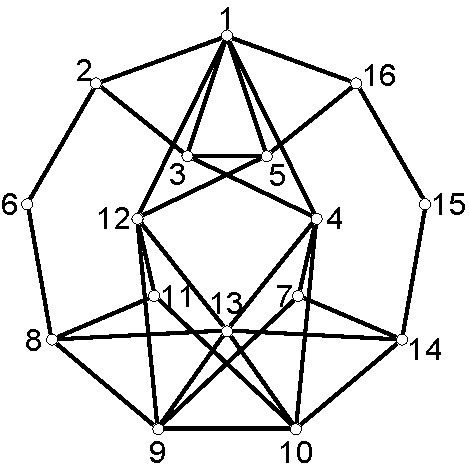
\includegraphics[scale=0.4]{i3322.pdf}
\caption{\label{Fig7}Exclusivity graph associated to $I_{3322}^{\rm BL}$.
The events are: \add{(do event come without parentheses?)}
 1: $1,1|2,2$,
 2: $0,0|2,0$,
 3: $1,0|2,2$,
 4: $0,0|2,1$,
 5: $0,1|2,2$,
 6: $\_,1|\_,0$,
 7: $\_,1|\_,1$,
 8: $0,0|1,0$,
 9: $1,0|1,1$,
10: $0,1|1,1$,
11: $1,\_|1,\_$,
12: $0,0|1,2$,
13: $1,1|1,1$,
14: $0,0|0,1$,
15: $1,\_|0,\_$, and
16: $0,0|0,2$.}
\end{figure}


For the exclusivity graph (Fig.~\ref{Fig7}) associated with Bell inequality $I_{3322}^{\rm BL}\leq 6$,
we can construct a NC inequality with the form\add{~\cite{cabello16}}
\begin{align}
I_{3322}^{\rm QC}
&=\sum_{i\in V}P_{|\psi\rangle}(A_i=1)-\sum_{(i,j)\in E}P_{|\psi\rangle}(A_i=1,A_j=1)\nonumber\\
&\overset{{\rm{NCHV}}}\leq 6,
\label{I3322QC}
\end{align}
where $V$ and $E$, respectively, denote the vertex and edge sets of the graph $G(V,E)$ in \replace{FIG}{Fig}. \ref{Fig7},
$P_{|\psi\rangle}(A_i=1)$ denotes the probability of obtaining result 1 when the observable $|A_i\rangle\langle A_i|$ is measured on the state $|\psi\rangle $,  i.e., $P_{|\psi\rangle}(A_i=1)= |\langle \psi|A_i\rangle|^2$, $P_{|\psi\rangle}(A_i=1,A_j=1)$, i.e.,  $P_{|\psi\rangle}(A_i=1)P_{|\psi\rangle}(A_j=1)$, represents experimental imprecision \replace{when}{of} $|A_i\rangle\bot |A_j\rangle$\replace{, i.e.,}{when} vertex $i$ and vertex $j$ are connected in FIG. \ref{Fig7}.

\emph{Remark 1}---The maximal quantum contextuality of  $I_{3322}^{\rm QC}$  is the Lov\'asz number of graph $G(V,E)$, i.e., $6.58841287$, achieved with systems of dimension five. See \cite{SM} for the \replace{optical}{optimal} settings and the state.


To detect the phenomenon of quantum contextuality beyond Bell nonlocality, we focus on 
 the four-dimensional system, in which the maximal quantum contextuality of $I_{3322}^{\rm QC}$ is about $6.57152.$ The \replace{optical}{optimal} settings and the state are listed in Table~\ref{numerica3}. The difference of maximum  $I_{3322}^{\rm QC}$ and maximum $I_{3322}^{\rm BL}$ is larger than $0.3$.

\begin{table}[htbp]
\centering
  \begin{tabular}{lccccc} \hline \hline
$|A_i\rangle$ & $i_1$ & $i_2$ & $i_3$ & $i_4$  \\
\hline
$|A_1\rangle$ & $0$ & $0$ & $1$ & $0$  \\
$|A_2\rangle$  & $0.469723$ & $0.453743$ & $0$ & $0.757283$  \\
$|A_3\rangle$ & $0.746839$ & $0.253161$ & $0$ & $0.614931$  \\
$|A_4\rangle$  & $0$ & $0.924703$ & $0$ & $-0.38069$  \\
$|A_5\rangle$ & $0.253161$ & $0.746839$ & $0$ & $-0.614931$  \\
$|A_6\rangle$ & $0.249899$ & $0.754381$ & $0$ & $0.607009$  \\
$|A_7\rangle$ & $1$ & $0$ & $0$ & $0$  \\
$|A_8\rangle$  & $0.924703$ & $0$ & $0$ & $-0.38069$  \\
$|A_9\rangle$  & $0$ & $1$ & $0$ & $0$  \\
$|A_{10}\rangle$  & $1$ & $0$ & $0$ & $0$ \\
$|A_{11}\rangle$ & $0$ & $1$ & $0$ & $0$  \\
$|A_{12}\rangle$  & $0.924703$ & $0$ & $0$ & $0.38069$  \\
$|A_{13}\rangle$  & $0$ & $0$ & $1$ & $0$  \\
$|A_{14}\rangle$  & $0$ & $0.924703$ & $0$ & $0.38069$  \\
$|A_{15}\rangle$ & $0.754381$ & $0.249899$ & $0$ & $-0.607009$  \\
$|A_{16}\rangle$  & $0.453743$ & $0.469723$ & $0$ & $0.757283$  \\
\hline
$|\psi\rangle$ & $\frac{1}{\sqrt{2}}$ & $\frac{1}{\sqrt{2}}$ & $0$ & $0$\\
  \hline \hline
   \end{tabular}
\caption{Numerical optimal settings and state for $I_{3322}^{\rm QC}$  in the four-dimensional system.}
\label{numerica3}
\end{table}

\begin{figure*}[htbp]
    \centering
    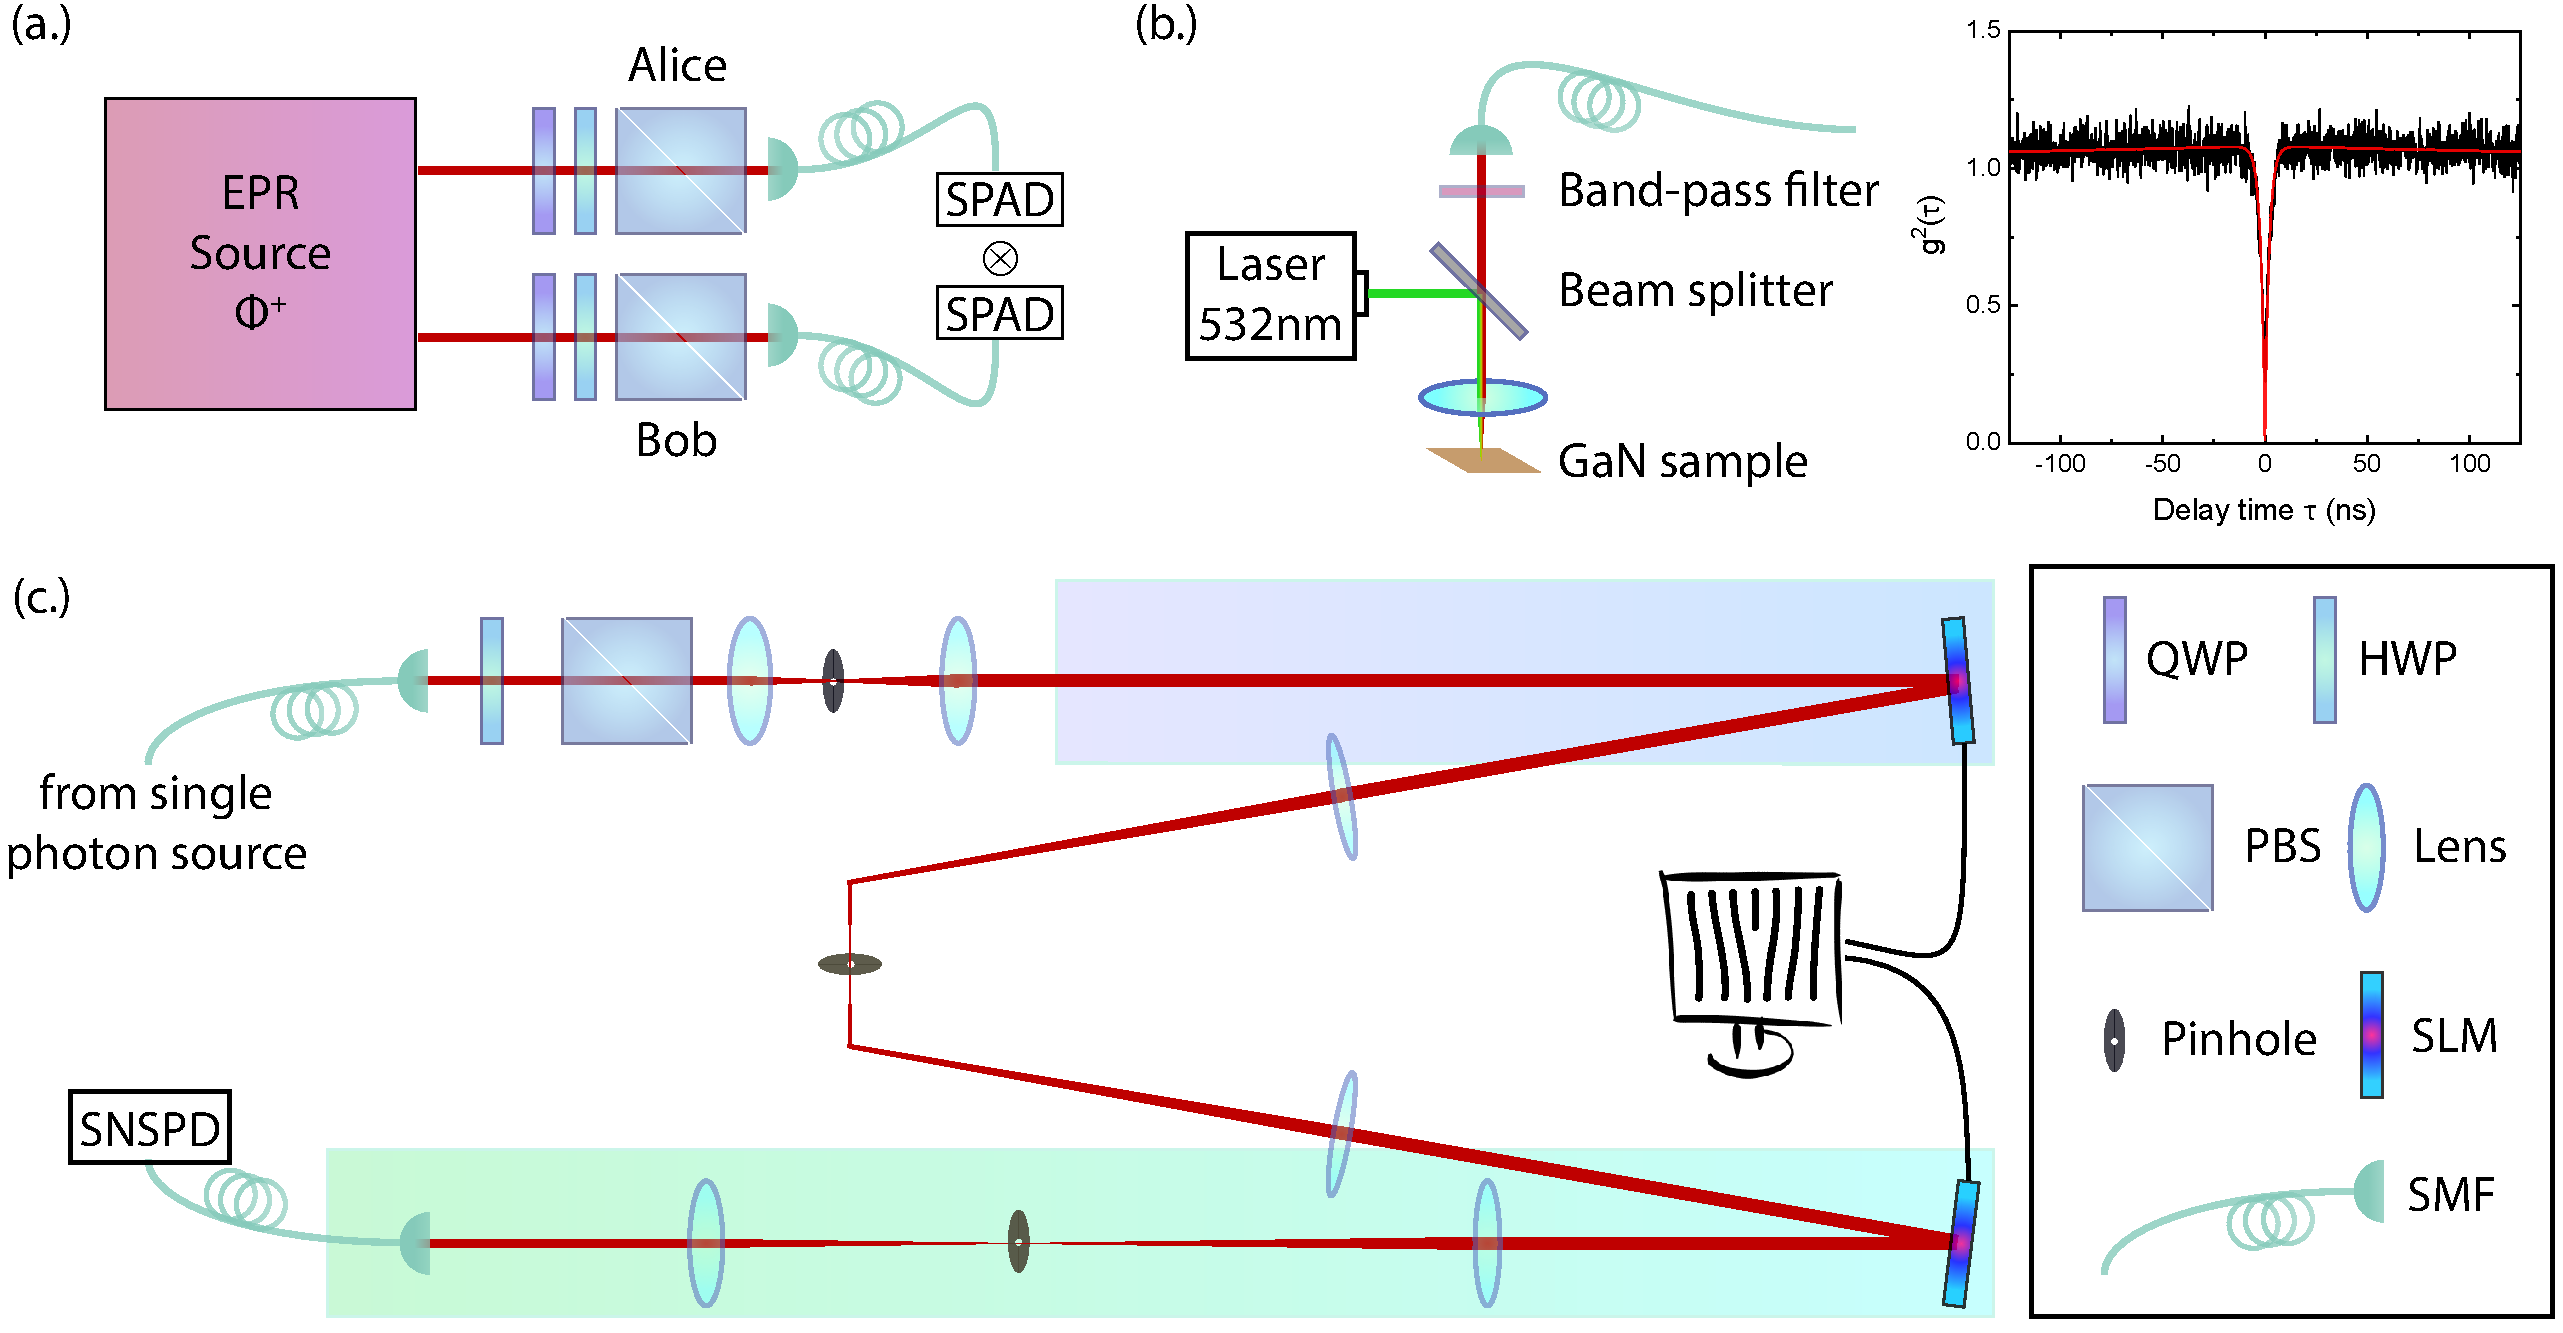
\includegraphics[width = .97\textwidth]{fig/exp-sch-draft-v2.pdf}
    \caption{Experimental setup.
    (a.) The two-particle setup to check the nonlocality inequation. Two maximally polarization-entangled photons were separately sent to Alice and Bob, going through their polarization discrimination system and recorded by single-photon avalanche detectors (SPAD) to perform 3-settings, 2-outcomes coincidence measurement.
    (b.) The single photon source, prepared by exciting an intrinsic defect in a bulk GaN sample. The second-order photon correlation function at zero delay without background correction was 0.225, clearly exhibiting the signature of photon antibunching and confirmed the character of single-photon emission. Single photons emitted were further filtered by a band-pass filter with a central wavelength of 780 nm and a bandwidth of 25 nm, and sent to the contextuality test setup.
    (c.) The single-body contextuality test setup.
    %Single photons filtered by a single mode optical fiber (SMF) were sent to the setup.     The polarization of single photon was prepared by a half-wave plate (HWP) and a polarization beam splitter (PBS).
    The single photons from (b), after passing through the beam expanding system with two lenses and a pinhole between them, were sent to a spatial light modulator (SLM) controlled by a computer to prepared the high-dimensional states, which is denoted by an violet box. The measurement setup located in the teal box consists of another SLM and SMF, and the counting apparatus here was a superconducting nanowire single-photon detector (SNSPD).}
    \label{fig:exp-sch}
 \end{figure*}

\emph{Remark 2}---For the above settings and state, the orthogonal relationship can be satisfied with errors \replace{$10^{-32}$}{of $10^{-32}$ magmitude}, i.e.,
$\sum_{(i,j)\in E}P_{|\psi\rangle}(A_i=1,A_j=1)\approx 9.62965\times 10^{-33}<10^{-32}.$
In fact, there exist settings and state (\cite{SM}) such that the orthogonal relationship is strictly satisfied  $(\sum_{(i,j)\in E}P_{|\psi\rangle}(A_i=1,A_j=1)=0)$ and $\max I_{3322}^{\rm QC}\approx 6.56233.$ 

Since the quantum system we utilize in experiment is four dimensional, we need extend the graph with extra projectors to construct full sets of compatible observables, such that every projector is measured as part of a complete basis \cite{yxiao17}. By Table~\ref{numerica3}, we only need to measure with the following six complete bases:
\begin{eqnarray}
\left\{
  \begin{array}{ll}
    \{|A_1\rangle,|A_2\rangle,|A_3\rangle,|A_{17}\rangle\},  \{|A_1\rangle,|A_4\rangle,|A_7\rangle,|A_{18}\rangle\},\\
\{|A_1\rangle,|A_{5}\rangle,|A_{16}\rangle,|A_{19}\rangle\},
\{|A_1\rangle,|A_{9}\rangle,|A_{12}\rangle,|A_{20}\rangle\},\ \ \ \\
\{|A_{6}\rangle,|A_{8}\rangle,|A_{21}\rangle,|A_{22}\rangle\},
\{|A_{14}\rangle,|A_{15}\rangle,|A_{23}\rangle,|A_{24}\rangle\},
\end{array}
\right.
\end{eqnarray}
where $|A_{21}\rangle$ and $|A_{23}\rangle$ can be taken as $|A_{1}\rangle$ and $|A_{17}\rangle,|A_{18}\rangle,|A_{19}\rangle,|A_{20}\rangle,|A_{22}\rangle,|A_{24}\rangle$ are uniquely determined by their corresponding incomplete basis since the system we focus on is four-dimensional and the  all incomplete bases have three pairwise orthogonal vectors.
 Thus, the detection probability of each observable such as $|A_{2}\rangle\langle A_{2}|$ can be obtained as
\begin{eqnarray}
\begin{split}
&P_{|\psi\rangle}(A_2=1)=\\
&\frac{N_{|\psi\rangle}(A_2)}
{N_{|\psi\rangle}(A_1)+N_{|\psi\rangle}(A_2)+N_{|\psi\rangle}(A_2)+N_{|\psi\rangle}(A_{17})},
\end{split}
\end{eqnarray}
where $N_{|\psi\rangle}(A_i)$ is the number of counts of obtaining result 1 when the observable $|A_{i}\rangle\langle A_{i}|$ is measured on the state $|\psi\rangle.$

 
  \begin{figure*}[htbp]
     \centering
     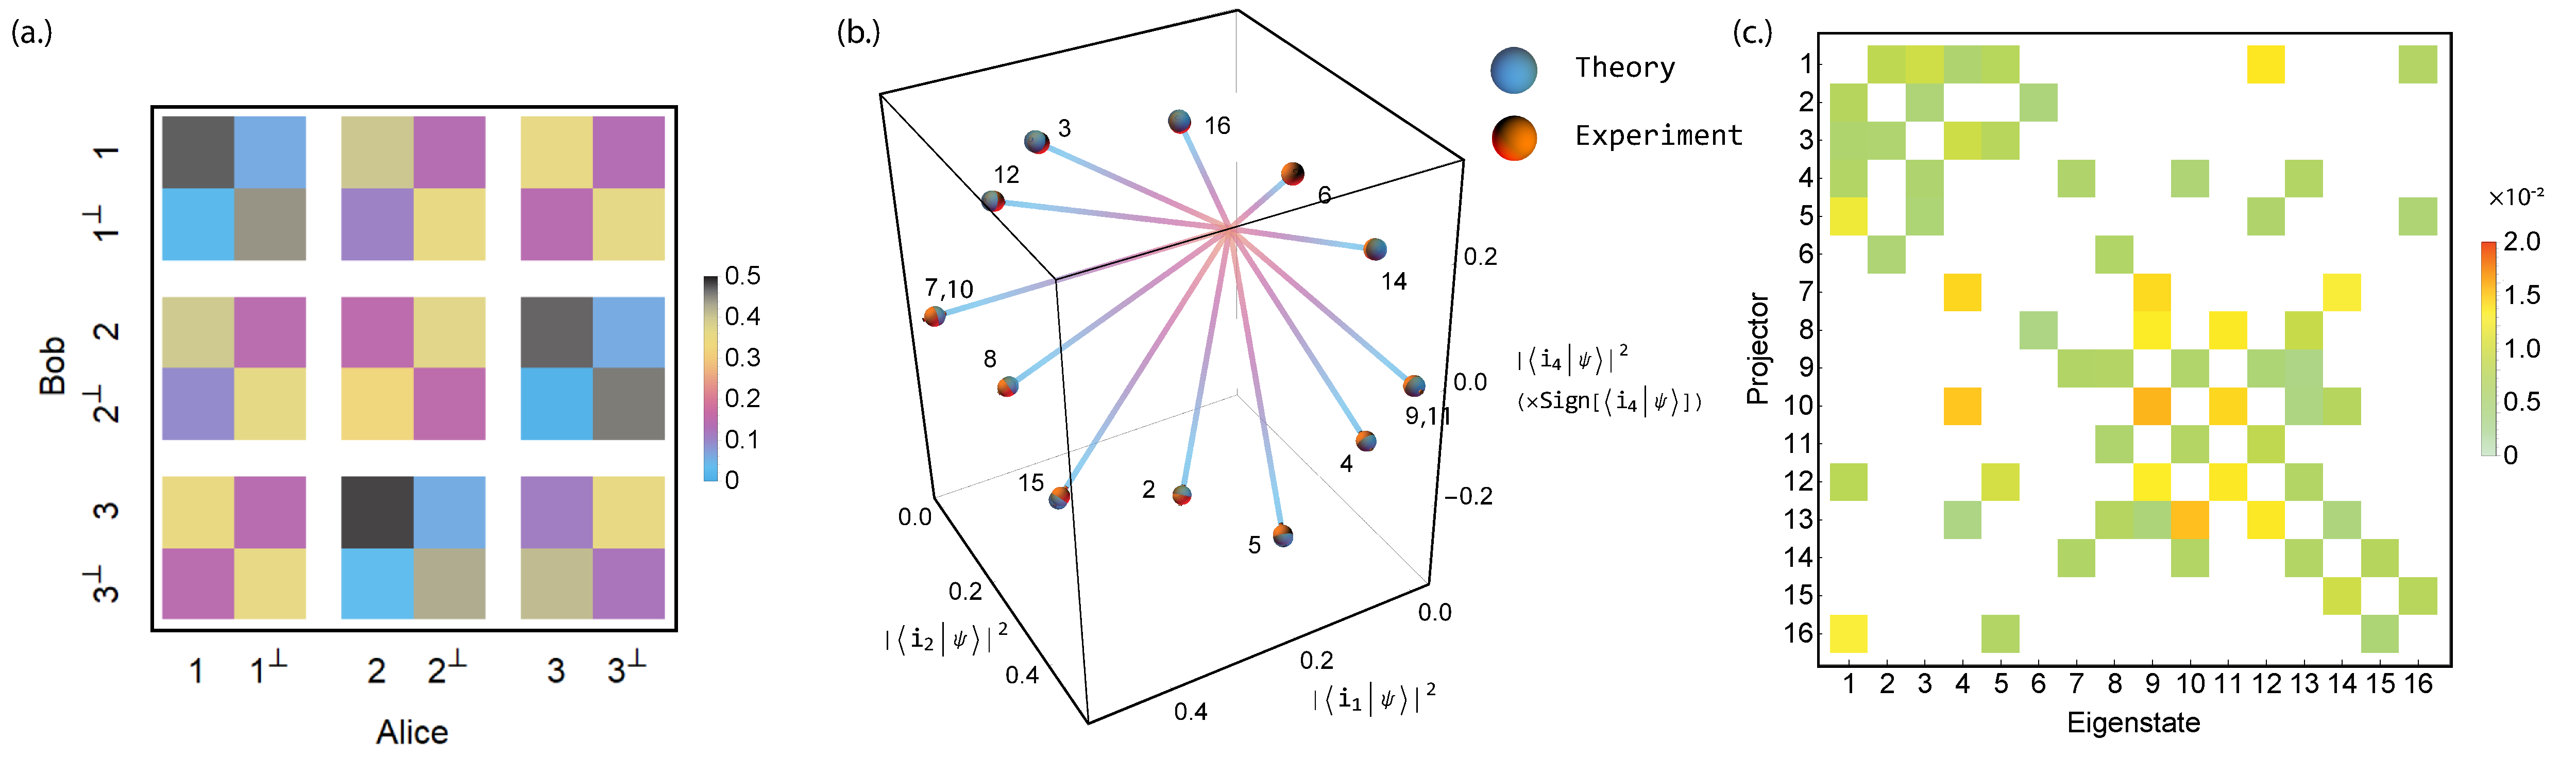
\includegraphics[width = .97 \textwidth]{fig/exp-res-all.pdf}
     \caption{Experimental results of detection probabilities for computing $I_{3322}^{BL}$ (a) and $I_{3322}^{QC}$ (b and c).
     (a.) Coincidence counting probabilities of Alice and Bob when they choose their optimal settings.
     (b.) Detection probabilities of the 16 optimal projectors, representing the 16 vertices of corresponding exclusivity graph, with the input state $|\Phi\rangle$.
     The dots are arranged in $(xyz)\to(|\braket{i_1|\psi}|^2, |\braket{i_2|\psi}|^2, \braket{i_4|\psi}|\braket{i_4|\psi}|)$ direction and the third dimension of $\braket{i_3|\psi}$ is omitted, so that $\braket{1|\psi}$ and $\braket{13|\psi}$ fall at the origin of Cartesian coordinate and are hidden, in which the experimental results also agree well with the theoretical prediction.
     (c.) Detection probabilities of unzero $P_{\ket{\alpha_i}}(\alpha_j)$, where eigenstates $\ket{\alpha_i}$ and projectors  $\ket{\alpha_j}$ are denoted by vertices, connected by 32 edges in the exclusivity graph.
     %In this plot, only the $32\times2$ blocks corresponding to 32 edges in the exclusivity graph are shown, irrelevant data whites out.
     }
     \label{fig:exp-res-all}
 \end{figure*}

 \emph{Experimental \replace{Part}{Setup and Result}---} 
 \delete{Theoretical model implies the $I_{3322}$ inequality has two distinct upper bounds, $I_{3322}^{\rm BL}\leq6.25$ and $I_{3322}^{\rm QC}\leq6.58$, corresponding to the maximal two-party nonlocal violation and single-body contextual violation, predicted by quantum theory respectively. In this Letter, we} We are now ready to experimentally test the two distinct upper bounds of $I_{3322}$ inequality, namely, $I_{3322}^{\rm BL}\leq6.25$ and $I_{3322}^{\rm QC}\leq6.58$ separately, to explicitly demonstrate quantum cpntextuality over Bell nonlocality. We start from $I_{3322}^{\rm BL}$. \replace{by virtue of}{Based on} a maximally entangled photonic polarization qubits, we checked the maximal violation \replace{of the nonlocal version of the inequality, namely,}{corresponding to} $I_{3322}^{\rm BL}$.
 A type-\rom{2} $\beta$-Barium borate ($\beta$-BBO) crystal was pumped by a frequency-doubled femtosecond laser to generate \delete{two} polarization-entangled \add{bi}photon\delete{s} \add{at intersections of the two spontaneous parametric down-conversion emission cones}, which were further sent to Alice and Bob, where a polarization beam splitter (PBS), proceeded by a quarter waveplate (QWP) and a half waveplate (HWP), was utilized to \replace{conduct the desired measurement settings}{construct a polarization discrimination system}.
 Two single-photon avalanche detectors (SPAD) recorded photon counting rate after the polarization discrimination system, and their coincidence counts was proportional to the probability of detecting two photons with a certain setting.
 
 %In the two-dimensional case, the setting to acquire maximal possible violation with two maximally entangled qubits $\ket{\Phi^+}$ have been worked out. More precisely, these settings are listed in table~\ref{tab:set3}. 
 In this experiment, the measurement settings were tuned by adjusting the angle of the quarter and half waveplates in the polarization discrimination system. For each set of measurement, the total photon count was about $8000$, and result was shown in Fig.~\ref{fig:exp-res-all}b. Substituting the measurement result into (\ref{I3322BL}) gives a result of $I_{3322}^{BL}(\ket{\Phi^+})=6.165 \pm 0.012$. Here, the errors were calculated according to the Poisson distribution, more precisely, by simulating the values of each measurement quantity from Poisson distribution for 100 randomly groups of counting sets, and taking the standard deviation of the simulated results as error. The result surpasses prediction of any possible LHV model but, due to imperfections in experiment, falls sightly below the qubit's Tsirelson bound $6.25$.

 We now turn to inspection of $I_{3322}^{\rm QC}$. \delete{Secondly, }In a 4-dimensional space, the single-body quantum contextual violation of the inequality, $I_{3322}^{\rm QC}$ was checked.
 To construct this synthetic space, we exploit the capability of the orbital angular momentum (OAM) of light. \replace{Apart from polarization}{Unlike photon's polarazation which is a homomorphic of a two-state system}, OAM ideally \replace{offers freedom to construct}{spans} an infinite dimension \delete{of synthetic} space\add{, and the eigenstates with lower winding numbers allow precise manipulation}. 
 4 eigenvectors, namely, $\ket{i_1} = \ket{1}, \ket{i_2} = \ket{3}, \ket{i_3} = \ket{-1}$, and $\ket{i_4} = \ket{-3}$, were selected within the photonic OAM degree of freedom. The manipulation of states was accomplished by modulating the phase of the photon's wavefunction.

 By exciting an intrinsic defect in a bulk GaN sample, we obtained an ultrabright, photostable single-photon sources at room temperature~\cite{qli18}. 
 A band-pass filter with a central wavelength of 780 nm and a width of 25 nm was inserted to filter the fluorescence of the defects and match the operation wavelength of the contextuality test setup. The total photon counting rate post the filter was about $0.94M$cps.

 The single photon was directed to the setup by a single-mode fiber (SMF), and spatial-filtered into fundamental Gaussian mode.
 Using a spatial light modulator (SLM), a coordinate-related wavefunction, determined by holograms displayed on the SLM, was bestowed to photons.
 \delete{The method reported in ~\cite{bolduc13} was adopted to ensure simultaneous and precise control of amplitude and phase in first order of diffraction.}
 The photons would then carry a wavefunction resembling superpositions of Laguerre-Gaussian modes $LG_p^l$ with OAM number of $l$~\cite{allen92} and be prepared to desired initial 4-dimension states $\ket{\psi}$, after being diffracted by the first SLM.
 A $4f$ system mapped the first and the second SLM at its input and output plane, with an aperture inserted at the focal plane to filter off the unwanted zero- and higher-order diffraction terms.
 The second SLM converted specific basis $\ket{\alpha}$ back to $\ket{0}$, which was post-selected by an SMF, as photons carrying nonzero OAM cannot be focused to a spot and collected by an SMF.
 In addition, a telescope lens was inserted between the second SLM and SMF to adjust beam size and optimize fiber coupling effeciency.
 Photons were then sent to a superconducting nanowire single-photon detector (SNSPD), where the counting rate would be proportional to the probability of projection measurements, i.e., $\left|\braket{\alpha|\psi}\right|^2$.
 
 The input state was prepared to be $\ket{\psi} = (\ket{i_1}+\ket{i_2})/\sqrt{2}$, and the 16 corresponding projectors $\bra{A_j}, j\in1..16$ were then measured on 6 sets of complete bases.
 We further considered the experimental imperfections. Orthogonality of states represented by connected vertices in the exclusivity graph was tested, and their effects were subtracted from the inequality, yielding the second term of $I_{3322}^{\rm QC}$. 
 To test the inequality~\ref{I3322QC}, we also need to check the no-signaling condition, \add{which requires the local marginal probabilities of successive measurements to be irrelavent to the other settings, forward or backward in time, being choosed, as suggested in~\cite{cabello16}.} See~\cite{SM} for detailed information of this test.

 The first term of $I_{3322}^{QC}$ inequality was evaluated by directly referring to detect probabilities of the 16 corresponding projectors on $6$ full sets of compatible observables. In order to obtain all probabilities needed for the exclusivity graph, there were 19 independent projectors in total.
 % And these projectors made six sets of complete bases, namely, $\{| 1\rangle,| 2\rangle,| 3\rangle,| {17}\rangle\}, \{| 1\rangle,| 4\rangle,| 7\rangle,| {18}\rangle\}, \{| 1\rangle,| {5}\rangle,| {16}\rangle,| {19}\rangle\}, \{| 1\rangle,| {9}\rangle,| {12}\rangle,| {20}\rangle\}, \{| {6}\rangle,| {8}\rangle,| {21}\rangle,| {22}\rangle\}, \text{ and } \{| {14}\rangle,| {15}\rangle,| {23}\rangle,| {24}\rangle\}$.
 Measurement settings of these projectors were shown in~\cite{SM}.
 The counting rate of each projector was then recorded and the detection probability was calculated. The integration time for each projection measurement was 10 seconds. Shown in Fig.~\ref{fig:exp-res-all}b, the results were fairly close to prediction.
 The numeric result of the first term of $I_{3322}^{QC}$ was $6.548 \pm 0.020$, error estimated by assuming Poisson distribution as \delete{was done} in the previous section.

\iffalse

\begin{table}[htbp]
    \centering
    \begin{tabular}{|c|cccc|} \hline \hline
$\ket{i}$ & $i_1$ & $i_2$ & $i_3$ & $i_4$  \\
\hline
$\ket{1}, \ket{13}, \ket{21}, \ket{23}$ & $0$ & $0$ & $1$ & $0$  \\
$|2\rangle$  & $0.469723$ & $0.453743$ & $0$ & $0.757283$  \\
$|3\rangle$ & $0.746839$ & $0.253161$ & $0$ & $0.614931$  \\
$|4\rangle$  & $0$ & $0.924703$ & $0$ & $-0.38069$  \\
$|5\rangle$ & $0.253161$ & $0.746839$ & $0$ & $-0.614931$  \\
$|6\rangle$ & $0.249899$ & $0.754381$ & $0$ & $0.607009$  \\
$\ket{7}, \ket{10}$ & $1$ & $0$ & $0$ & $0$  \\
$|8\rangle$  & $0.924703$ & $0$ & $0$ & $-0.38069$  \\
$\ket{9}, \ket{11}$  & $0$ & $1$ & $0$ & $0$  \\
$|12\rangle$  & $0.924703$ & $0$ & $0$ & $0.38069$  \\
$|14\rangle$  & $0$ & $0.924703$ & $0$ & $0.38069$  \\
$|15\rangle$ & $0.754381$ & $0.249899$ & $0$ & $-0.607009$  \\
$|16\rangle$  & $0.453743$ & $0.469723$ & $0$ & $0.757283$  \\
$\ket{17}$ & $0.470735$ & $-0.854416$ & $0$ & $-0.219958$ \\
$\ket{18}$ & $0$ & $0.38069$ & $0$ & $0.924703$ \\
$\ket{19}$ & $0.854416$ & $-0.470735$ & $0$ & $-0.219958$ \\
$\ket{20}$ & $0.38069$ & $0$ & $0$ & $-0.924703$ \\
$\ket{22}$ & $0.287185$ & $-0.656437$ & $0$ & $0.697578$ \\
$\ket{24}$ & $0.656437$ & $-0.287185$ & $0$ & $0.697578$ \\
\hline
$|\psi\rangle$ & $1/\sqrt{2}$ & $1/\sqrt{2}$ & $0$ & $0$ \\
  \hline \hline
   \end{tabular}
    \caption{Measurement settings for $I_{3322}^{QC}$ in four-dimensional systems to acquire maximal violation against NCHV models.}
    \label{tab:set19}
 \end{table}

\fi

 The second term of $I_{3322}^{\rm QC}$ inequality which represents experimental imperfections of orthogonality between states denoted by connected vertices in the exclusivity graph.
 Similar as the way the first term was calculated, the second term was also evaluated by adding up mutual projection probabilities of the states mentioned above, and their fluctuation also estimated by Poisson distribution, yielding a value of $-0.060 \pm 0.005$ without correcting background noise from SNSPD and stray light.

 By adding the two terms together, the final result of $I_{3322}^{\rm QC}$ turned out to be $6.488 \pm 0.025$, exceeding the classical bound by about 19 standard deviations and the Tsirelson bound derived from Bell nonlocality by over 9 standard deviations. \replace{This result supports that for the $I_{3322}$ case, a high violation from any non-contextual hidden variable model exists, which cannot be explained by nonlocality per se, and has to be accounted for by quantum contextuality.}{We thus successfully observed the quantum contextuality beyond Bell nonlocality's bounud.}

 \emph{Conclusion and Discussion.}--- \add{The inequality approach is a lucid method to describe the degree how contextual and nonlocal QT is. By virtue of graph theory, connections between quantum contextuality and graph's characteristic Lov\'asz number is established.
 Following the CSW approach, we investigated the exclusivity graph which gives $I_{3322}$ inequality. 
 \replace{The optimal solution in 4-dimensional space was proposed to give maximal quantum contextuality correlation, and by}{By} removing the constraints of Bell-type experiment, for the $I_{3322}$ case a remarkably high violation from any non-contextual hidden variable model exists, which cannot be explained by nonlocality per se, and has to be accounted for by quantum contextuality. 
 The key point lays under this result is that, although quantum contextuality is stated without spacelike restriction, and may be considered a more weakened property than Bell nonlocality, it actually gives stronger prediction in some sense. 
 Our work indicate the deep-rooted connection between graph theory and physics, and is in turn beneficial for profound comprehension of the QT.
 }

%\begin{acknowledgments}
 \textit{Acknowledgement}.---This work was supported by the National Key Research and Development Program of China (Grant No. 2016YFA0302700), the National Natural Science Founda-tion of China (Grants No. 61725504, 61327901, 61490711 and 11774335), the Key Research Program of Frontier Sciences, Chinese Academy of Sciences (CAS) (Grant No. QYZDY-SSW-SLH003), Anhui Initiative in Quantum Information Technologies (AHY060300 and AHY020100), the Fundamental Research Funds for the Central Universities (Grant No. WK2470000020 and WK2470000026). J.L.C. is supported by National Natural Science Foundations of China (Grant No.\ 11475089).

 Z. H. L., H. X. M. and Z. P. X. contributed equally to this work.
%\end{acknowledgments}



\begin{thebibliography}{10}
%	\providecommand{\url}[1]{\texttt{#1}}
%	\providecommand{\urlprefix}{URL }
%	\providecommand{\eprint}[2][]{\url{#2}}
\bibitem{Specker60}
 E. P. Specker,
 %Die Logik nicht gleichzeitig entscheidbarer Aussagen.
 \href{http://onlinelibrary.wiley.com/doi/10.1111/j.1746-8361.1960.tb00422.x/abstract}{Dialectica \textbf{14}, 239 (1960).}

\bibitem{KS67}
 S. Kochen and E. P. Specker,
 %The problem of hidden variables in quantum mechanics.
 \href{http://www.iumj.indiana.edu/IUMJ/fulltext.php?year=1968&volume=17&artid=17004}{J. Math. Mech. \textbf{17}, 59 (1967).}

\bibitem{Bell66}
 J. S. Bell,
 %On the problem of hidden variables in quantum mechanics.
 \href{http://rmp.aps.org/abstract/RMP/v38/i3/p447_1}{Rev. Mod. Phys. \textbf{38}, 447 (1966).}

\bibitem{Bell64}
 J. S. Bell,
 Physics \textbf{1}, 195 (1964).

%%%%%%%%%%%%%%%%%%%%%%%%%%%%%%%%%%%%%%%%%%%%%%%%%%%%%%%%%%%%%%%%%%%

\bibitem{KCBS08}
 A. A. Klyachko, M. A. Can, S. Binicio\u{g}lu, and A. S. Shumovsky,
 %Simple Test for Hidden Variables in Spin-1 Systems
 \href{http://dx.doi.org/10.1103/PhysRevLett.101.020403}{Phys. Rev. Lett. \textbf{101}, 020403 (2008).}

\bibitem{Cabello08}
 A. Cabello,
 %Experimentally Testable State-Independent Quantum Contextuality.
 \href{http://dx.doi.org/10.1103/PhysRevLett.101.210401 }{Phys. Rev. Lett. \textbf{101}, 210401 (2008).}

%%%%%%%%%%%%%%%%%%%%%%%%%%%%%%%%%%%%%%%%%%%%%%%%%%%%%%%%%%%%%%%%%%%


%%%%%%%%%%%%%%%%%%%%%%%%%%%%%%%%%%%%%%%%%%%%%%%%%%%%%%%%%%%%%%%%%%%

\bibitem{Raussendorf13}
 R. Raussendorf,
 %Contextuality in measurement-based quantum computation.
 \href{http://link.aps.org/doi/10.1103/PhysRevA.88.022322}{Phys. Rev. A \textbf{88}, 022322 (2013).}

\bibitem{HWVE13}
 M. Howard, J. J. Wallman, V. Veitch, and J. Emerson,
 %Contextuality supplies the magic for quantum computation.
 \href{http://arxiv.org/abs/1401.4174}{\eprint{arXiv:1401.4174}.}

%%%%%%%%%%%%%%%%%%%%%%%%%%%%%%%%%%%%%%%%%%%%%%%%%%%%%%%%%%%%%%%%%%%

\bibitem{Ekert91}
 A. K. Ekert,
 %Quantum cryptography based on Bell's theorem.
 \href{http://journals.aps.org/prl/abstract/10.1103/PhysRevLett.67.661}{Phys. Rev. Lett. \textbf{67}, 661 (1991).}

\bibitem{CDNS11}
 A. Cabello, V. D'Ambrosio, E. Nagali, and F. Sciarrino,
 %Hybrid ququart-encoded quantum cryptography protected by Kochen-Specker contextuality.
 \href{http://journals.aps.org/pra/abstract/10.1103/PhysRevA.84.030302}{Phys. Rev. A \textbf{84}, 030302(R) (2011).}

%%%%%%%%%%%%%%%%%%%%%%%%%%%%%%%%%%%%%%%%%%%%%%%%%%%%%%%%%%%%%%%%%%%

\bibitem{BZPZ04}
 \v{C}. Brukner, M. \.{Z}ukowski, J.-W. Pan, and A. Zeilinger,
 %Bell's inequalities and quantum communication complexity.
 \href{http://journals.aps.org/prl/abstract/10.1103/PhysRevLett.92.127901}{Phys. Rev. Lett. \textbf{92}, 127901 (2004).}

\bibitem{BCMW10}
 H. Buhrman, R. Cleve, S. Massar, and R. de Wolf,
 %Nonlocality and communication complexity.
 \href{http://journals.aps.org/rmp/abstract/10.1103/RevModPhys.82.665}{Rev. Mod. Phys. \textbf{82}, 665 (2010).}

%%%%%%%%%%%%%%%%%%%%%%%%%%%%%%%%%%%%%%%%%%%%%%%%%%%%%%%%%%%%%%%%%%%

\bibitem{PAMBMMOHLMM10}
 S. Pironio, A. Ac\'{\i}n, S. Massar, A. Boyer de la Giroday,
 D. N. Matsukevich, P. Maunz, S. Olmschenk, D. Hayes, L. Luo, T. A. Manning, and C. Monroe,
 %Random numbers certified by Bell's theorem.
 \href{http://www.nature.com/nature/journal/v464/n7291/full/nature09008.html}{Nature (London) \textbf{464}, 1021 (2010).}

\bibitem{UZZWYDDK13}
 M. Um, X. Zhang, J. Zhang, Y. Wang, S. Yangchao, D.-L. Deng, L.-M. Duan, and K. Kim,
 %Experimental certification of random numbers via quantum contextuality.
 \href{http://www.nature.com/srep/2013/130409/srep01627/full/srep01627.html}{Sci. Rep. \textbf{3}, 1627 (2013).}

%%%%%%%%%%%%%%%%%%%%%%%%%%%%%%%%%%%%%%%%%%%%%%%%%%%%%%%%%%%%%%%%%%%


\bibitem{CSW10}
 A. Cabello, S. Severini, and A. Winter,
 %(Non-)Contextuality of physical theories as an axiom.
 \href{http://arxiv.org/abs/1010.2163}{\eprint{arXiv:1010.2163}.}

\bibitem{CSW14}
 A. Cabello, S. Severini, and A. Winter,
 %Graph-theoretic approach to quantum correlations
 \href{http://journals.aps.org/prl/abstract/10.1103/PhysRevLett.112.040401}{Phys. Rev. Lett. \textbf{112}, 040401 (2014).}
 
\bibitem{Pal10} 
 K.F. P\'al and T. V\'ertesi,
 %Maximal violation of the I3322 inequality using infinite dimensional quantum systems.
 \href{https://dx.doi.org/10.1103/PhysRevA.82.022116}{\eprint{Phys. Rev. A 82, 022116 (2010)}.}
 
\bibitem{SBBC13}
 M. Sadiq, P. Badzi{\c a}g, M. Bourennane, and A. Cabello,
 %Bell inequalities for the simplest exclusivity graph.
 \href{http://pra.aps.org/abstract/PRA/v87/i1/e012128}{Phys. Rev. A \textbf{87}, 012128 (2013).}

%%%%%%%%%%%%%%%%%%%%%%%%%%%%%%%%%%%%%%%%%%%%%%%%%%%%%%%%%%%%%%%%%%%




\bibitem{BG08}
 N. Brunner and N. Gisin,
 %Partial list of bipartite Bell inequalities with four binary settings.
 \href{http://dx.doi.org/10.1016/j.physleta.2008.01.052}{Phys. Lett. A \textbf{372}, 3162 (2008).}

\bibitem{RDLTC14}
 R. Rabelo, C. Duarte, A. J. L\'opez-Tarrida, M. Terra Cunha, and A. Cabello,
 %Multigraph approach to quantum nonlocality.
 J. Phys. A (to be published).

\bibitem{SM}
 Supplemental Information for ``Experimental test of quantum contextuality beyond Bell nonlocality''.

\bibitem{cabello16}
 A.~Cabello,
 %Simple method for experimentally testing any form of quantum contextuality,
 Phys.~Rev.~A, \textbf{93}, 032102 (2016).

\bibitem{yxiao17}
 Y.~Xiao, Z.-P.~Xu, Q.~Li, J.-S.~Xu, K.~Sun, J.-M.~Cui, Z.-Q.~Zhou, H.-Y.~Su, A.~Cabello, J.-L.~Chen, C.-F.~Li, and G.-C.~Guo,
 %Experimental observation of quantum state-independent contextuality under no-signaling conditions,
 Opt.~Express \textbf{26} 38 (2018).
 
 \bibitem{qli18}
 Q.~Li, et al.,
 %Experimental simulation of anti-parity-time symmetric Lorentz dynamics,
 Optica \textbf{6}(1), 67 (2019)

% \bibitem{bolduc13}
% E.~Bolduc, N.~Bent, E.~Santamato, E.~Karimi, and R.~W.~Boyd,
% Exact solution to simultaneous intensity and phase encryption with a single phase-only hologram,
% Opt.~Lett. \textbf{38}, 3546 (2013).

 \bibitem{allen92}
 L.~Allen, M.~W.~Beijersbergen, R.~J.~C.~Spreeuw, and J.~P.~Woerdman,
 %Orbital angular momentum of light and the transformation of Laguerre-Gaussian laser modes,
 Phys.~Rev.~A \textbf{45}, 8185 (1992).

 %\bibitem{mair01}
 %A.~Mair, A.~Vaziri, G.~Weihs, and A.~Zeilinger,
 %Entanglement of the orbital angular momentum states of photons,
 %Nature \textbf{412} 313 (2001).







\end{thebibliography}


\end{document}



